
% \tikzstyle{int}=[draw, fill=blue!20, minimum size=2em]
% \tikzstyle{block}=[draw, fill=gray, minimum size=1.5em]
% \tikzstyle{init} = [pin edge={to-,thin,black}]
% 	\resizebox{8cm}{1.2cm}{
% \begin{tikzpicture}[node distance=1.5cm,auto,>=latex']
%     \node [block] (o) {};
%     \node (p) [left of=o,node distance=0.5cm, coordinate] {o};
%     \node [shape=circle,int] (a) [right of=o]{$A$};
%     \node (b) [left of=a,node distance=1.5cm, coordinate] {a};
%     \node [shape=circle,int] (c) [right of=a] {$B$};
%     \node (d) [left of=c,node distance=1.5cm, coordinate] {c};
%     \node [shape=circle,int, pin={[init]above:$$}] (e) [right of=c]{$C$}; 
%     \node (f) [left of=e,node distance=1.5cm, coordinate] {e};
%     \node [shape=circle,int] (g) [right of=e] {$D$};
%     \node (h) [left of=g,node distance=1.5cm, coordinate] {g};
%     \node [shape=circle,int] (i) [right of=g] {$E$};
%     \node (j) [left of=i,node distance=1.5cm, coordinate] {i};
%     \node [block] (k) [right of=i] {};
%     \node (l) [left of=k,node distance=0.5cm, coordinate] {k};

%     \path[<-] (o) edge node {$0$} (a);
%     \path[<->] (a) edge node {$0$} (c);
%     \path[<->] (c) edge node {$0$} (e);
%     \path[<->] (e) edge node {$0$} (g);
%     \path[<->] (g) edge node {$0$} (i);
%     \draw[->] (i) edge node {$1$} (k);
% \end{tikzpicture}
% }
\tikzstyle{int}=[draw, fill=blue!20, minimum size=2em]
\tikzstyle{block}=[draw, fill=gray, minimum size=1.5em]
\tikzstyle{init} = [pin edge={to-,thin,black}]

\resizebox{5cm}{1cm}{
    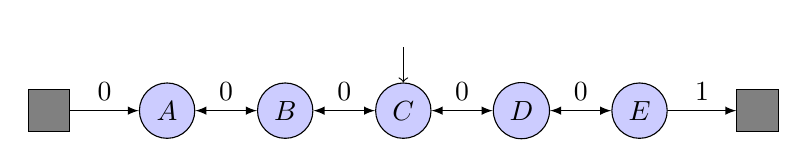
\begin{tikzpicture}[node distance=1.5cm, auto, >=latex]
        \node [block] (o) {};
        \node (p) [left of=o, node distance=0.5cm, coordinate] {o};
        \node [shape=circle, int] (a) [right of=o] {$A$};
        \node (b) [left of=a, node distance=1.5cm, coordinate] {a};
        \node [shape=circle, int] (c) [right of=a] {$B$};
        \node (d) [left of=c, node distance=1.5cm, coordinate] {c};
        \node [shape=circle, int, pin={[init]above:$ $}] (e) [right of=c] {$C$};
        \node (f) [left of=e, node distance=1.5cm, coordinate] {e};
        \node [shape=circle, int] (g) [right of=e] {$D$};
        \node (h) [left of=g, node distance=1.5cm, coordinate] {g};
        \node [shape=circle, int] (i) [right of=g] {$E$};
        \node (j) [left of=i, node distance=1.5cm, coordinate] {i};
        \node [block] (k) [right of=i] {};
        \node (l) [left of=k, node distance=0.5cm, coordinate] {k};

        \path[->] (o) edge node {$0$} (a);
        \path[<->] (a) edge node {$0$} (c);
        \path[<->] (c) edge node {$0$} (e);
        \path[<->] (e) edge node {$0$} (g);
        \path[<->] (g) edge node {$0$} (i);
        \draw[->] (i) edge node {$1$} (k);
    \end{tikzpicture}
}


  
    